% T402 Threat Model Diagram - Standalone TikZ
% Compile with: pdflatex threat-model.tex

\documentclass[tikz,border=10pt]{standalone}
\usepackage{tikz}
\usetikzlibrary{arrows.meta, shapes.geometric, positioning, calc, fit, backgrounds}
\usepackage{xcolor}

% Define colors
\definecolor{t402blue}{HTML}{3B82F6}
\definecolor{t402green}{HTML}{10B981}
\definecolor{t402purple}{HTML}{8B5CF6}
\definecolor{t402gray}{HTML}{6B7280}
\definecolor{t402orange}{HTML}{F59E0B}
\definecolor{t402red}{HTML}{EF4444}

\begin{document}
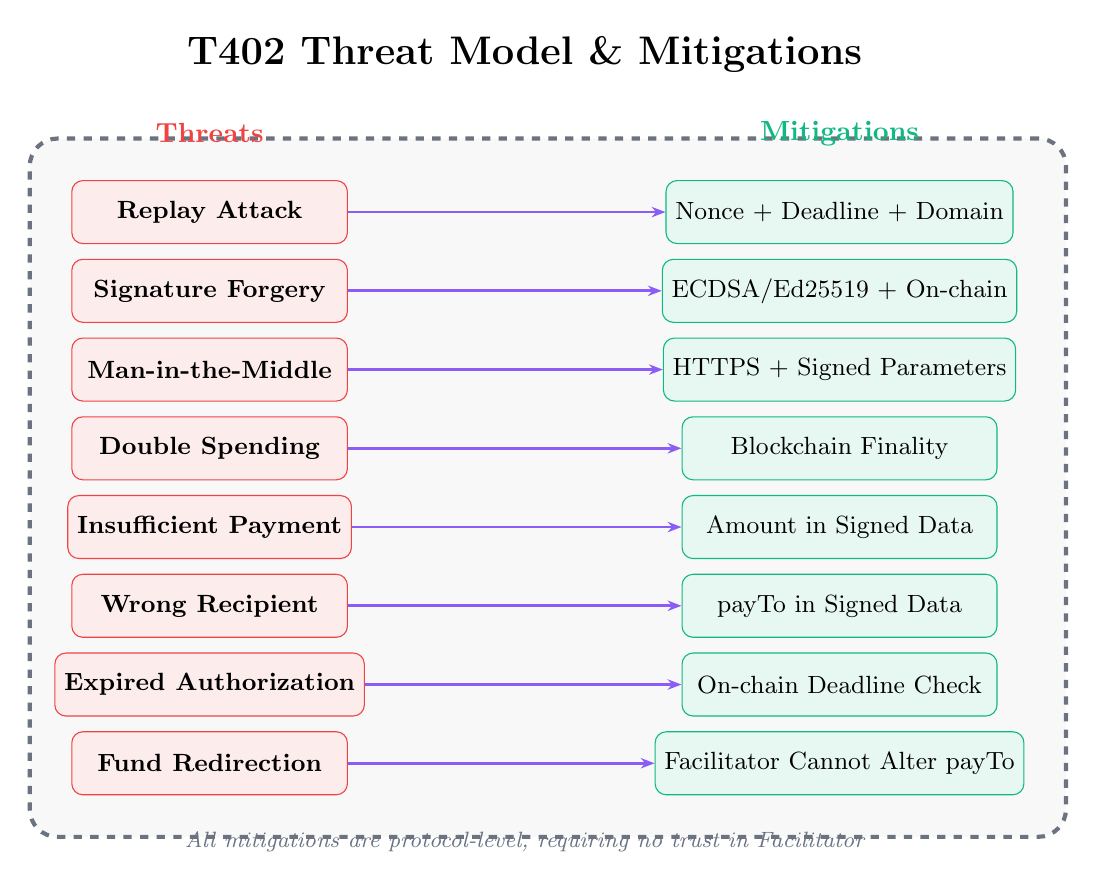
\begin{tikzpicture}[
    threat/.style={
        rectangle,
        rounded corners=4pt,
        minimum width=3.5cm,
        minimum height=0.8cm,
        draw=t402red,
        fill=t402red!10,
        font=\small\bfseries
    },
    mitigation/.style={
        rectangle,
        rounded corners=4pt,
        minimum width=4cm,
        minimum height=0.8cm,
        draw=t402green,
        fill=t402green!10,
        font=\small
    },
    arrow/.style={
        ->,
        >={Stealth[length=5pt]},
        line width=1pt,
        t402purple
    }
]

% Title
\node[font=\bfseries\Large] at (4,6.5) {T402 Threat Model \& Mitigations};

% Headers
\node[font=\bfseries, t402red] at (0,5.5) {Threats};
\node[font=\bfseries, t402green] at (8,5.5) {Mitigations};

% Threat-Mitigation pairs
\node[threat] (t1) at (0,4.5) {Replay Attack};
\node[mitigation] (m1) at (8,4.5) {Nonce + Deadline + Domain};
\draw[arrow] (t1) -- (m1);

\node[threat] (t2) at (0,3.5) {Signature Forgery};
\node[mitigation] (m2) at (8,3.5) {ECDSA/Ed25519 + On-chain};
\draw[arrow] (t2) -- (m2);

\node[threat] (t3) at (0,2.5) {Man-in-the-Middle};
\node[mitigation] (m3) at (8,2.5) {HTTPS + Signed Parameters};
\draw[arrow] (t3) -- (m3);

\node[threat] (t4) at (0,1.5) {Double Spending};
\node[mitigation] (m4) at (8,1.5) {Blockchain Finality};
\draw[arrow] (t4) -- (m4);

\node[threat] (t5) at (0,0.5) {Insufficient Payment};
\node[mitigation] (m5) at (8,0.5) {Amount in Signed Data};
\draw[arrow] (t5) -- (m5);

\node[threat] (t6) at (0,-0.5) {Wrong Recipient};
\node[mitigation] (m6) at (8,-0.5) {payTo in Signed Data};
\draw[arrow] (t6) -- (m6);

\node[threat] (t7) at (0,-1.5) {Expired Authorization};
\node[mitigation] (m7) at (8,-1.5) {On-chain Deadline Check};
\draw[arrow] (t7) -- (m7);

\node[threat] (t8) at (0,-2.5) {Fund Redirection};
\node[mitigation] (m8) at (8,-2.5) {Facilitator Cannot Alter payTo};
\draw[arrow] (t8) -- (m8);

% Security boundary
\begin{scope}[on background layer]
    \node[rectangle, rounded corners=10pt, draw=t402gray, dashed, line width=1.5pt,
          fit=(t1)(t8)(m1)(m8), inner sep=15pt, fill=t402gray!5] {};
\end{scope}

% Legend
\node[font=\footnotesize\itshape, t402gray] at (4,-3.5) {All mitigations are protocol-level, requiring no trust in Facilitator};

\end{tikzpicture}
\end{document}
